\section{Lezione 2016-10-20}
\subsection{TODO}
% Insert what you need. Any row is associated with the improvment or mistake
% arise. In the first column you can insert what you should resolve or change,
% instead in the second column you may put the section where to apply some
% modification.
\begin{table}[ht]
\begin{center}
\begin{tabular}{|p{\textwidth}|c|}
\hline
\multicolumn{1}{|c|}{\textbf{Miglioramento}} & \textbf{Sezione} \\ \hline
Far luce sul significato di \textit{dummy sinthesized attribute} &
\ref{sec:evaluation_order} \\ \hline
\end{tabular}
\end{center}
\caption{Tabella miglioramenti}
\label{tab:tab_todo}
\end{table}

\subsection{Syntax-Directed Translation}
Tecniga generale per la "manipolazione" dei programmi, basta sulla grammatica
libera dal contesto. La translazione \`e fortemente legata al parsing. Viene
utilizzata per l'\textbf{analisti statica} e la \textbf{generazione di codice}
ma anche in tutta una serie di altre attivit\`a
\begin{itemize}
\item genereazione di un \textit{abstract syntax tree}
\item valutazione di un'espressione
\item implementazione di \textit{Domain Specific Language}
\end{itemize}

\subsection{Syntax-Directed Definition}
\begin{definition}[Syntax-Directed]
Una syntex-directed definition (o attribute grammar) \`e una
\textbf{context-free grammar} dove
\begin{itemize}
\item gli attributi dei i terminali e non-terminali posseggono valori
\item alle produzione sono associate regole semantiche, il quale definisce il
valore degli attributi
\end{itemize}
\end{definition}

\paragraph{Valori}
Si annota il valore $val$ di un attributo $X$ come $$X.val$$
\paragraph{Regole semantiche}
La regola semantica di un produzione $A \to \alpha$ ha la forma
$$b:=f(c_1,c_2,...,c_k)$$
dove $b,c_1,c_2,...,c_k$ sono attributi di $A$ o dei simboli in $\alpha$.

\subsubsection{Attributi}
\begin{definition}[Annotated Parse Tree]
Un annotated parse tree \`e un \textbf{albero di parsing} dove tutti gli
attributi dei nodi hanno il corrispettivo valore.
\end{definition}

Gli attributi vanno a rappresentare tutte gli elementi fondamentali di un
programma:
\begin{itemize}
\item numeri (litterali costanti)
\item stringhe (litterali costanti)
\item rappresentazione intermedia di un programma
\begin{enumerate}
\item (puntatore ai) nodi dell'\textit{abstraxt syntax tree}
\item (puntatore alla) stringa rappresentate il codice intermedio
\end{enumerate}
\item locazioni di memoria
\item tipo del dato, valido il \textit{type checking} dell'espressione
\item informazioni di \textit{scoping} per dichiarazioni locali
\end{itemize}

Ogni simbolo della grammatica pu\`o avere un qualsiasi numero d'attributi.

\subsubsection{Attributi sintetici vs ereditati}
\begin{definition}[Synthesized and Inherited Attributes]
Data un produzione $A \to \alpha$ ed una regola semantica
$b:=f(c_1,c_2,...,c_k)$
\begin{itemize}
\item se $b$ \`e un attributo di $A$ allora \`e un attributo
\textbf{synthesized} di $A$
\item se $b$ \`e un attributo di un simbolo $B$ in $\alpha$ allora \`e un
attributo \textbf{inherited} di $B$
\end{itemize}
\end{definition}

I simbolo \textbf{terminali} hanno \textbf{solo} attributi \textbf{synthesized}.

Si prenda come esempio la grammatica che genera la dichiarazione dei tipi delle
variabili:
\begin{figure}[H]
  \centering
  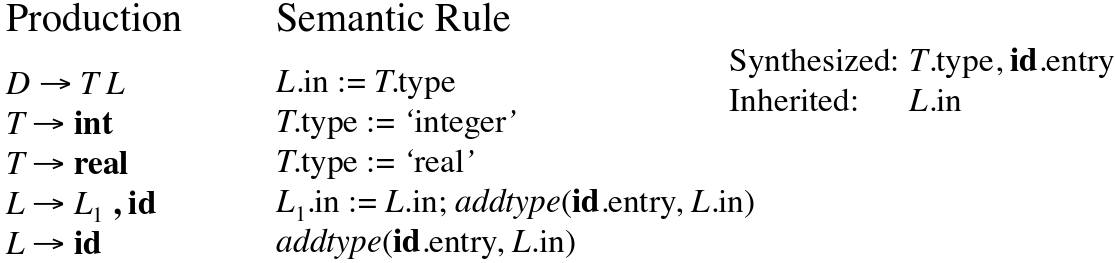
\includegraphics[scale=0.45]{res/image/ex_type}
  \caption{Esempio SDD con attributi \textit{synthesized} e \textit{inherited}}
  \label{img:ex_type}
\end{figure}

Come descritto in figura, $T.type$ \`e \textit{synthesized} in quanto attributo
del non-terminale della produzione corrispondente.
\begin{align*}
& {\color{red}T} \to \mathbf{real}  & {\color{red}T}.type:="real"
\end{align*}

Invece $L.in$ \`e un attributo \textit{inherited} perch\'e il non-terminale
appare all'interno della forma sentenziale della produzione.
\begin{align*}
& D \to T\color{red}L & {\color{red}L}.in:=T.type
\end{align*}

In fine, $\mathbf{id}.entry$ \`e \textit{synthesized} essendo l'attributo di un
terminale.

\begin{figure}[H]
  \centering
  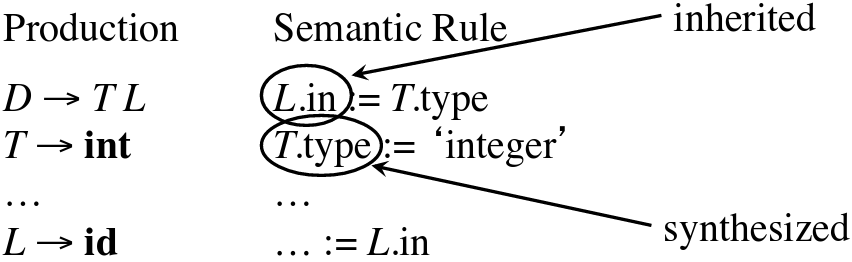
\includegraphics[scale=0.4]{res/image/synthesized_inherited}
  \caption{Attributi synthesized e inherited}
  \label{img:synthesized_inherited}
\end{figure}

Nelle regole semantiche (fig.\ref{img:ex_type}) gli attributi vanno ad
aggiungere alla tabella dei simboli informazione sul tipo delle variabili
attraverso un \textbf{limitato side-effect}.

La comodit\`a degli attributi \textit{inherited} \`e la gestione dell'
informazione che non rispetta la struttura ad albero.

\subsubsection{S-Attributed Definitions}
\begin{definition}[S-attributed definition]
Una syntax-directed definition che usa esclusivamente attributi synthesized \`e
chiamato S-attributed definition (o grammatica S-attributed).
\end{definition}

Un albero di parsing di una S-attribute definition pu\`o essere annotato con una
singola attraversata \textit{bottom-up}. Inoltre dato un albero di parsing un
qualsiasi algoritmo di attraversamento \textit{postorder depth-first} pu\`o
essere usato per \textbf{eseguire} regole semantiche e \textbf{assegnare}
attributi valore.

In alcuni casi gli attributi possono essere valutati durante il \textit{parsing}
senza costruire l'albero di parsing esplicitamente.

\subsubsection{Esempio Annoted Parse Tree}
Data la \textit{attribute grammar} in fig.\ref{img:sdd_example} e l'input
\textbf{9+5+2n} si va a costruire l'albero di parsing annotato.
\begin{figure}[H]
  \centering
  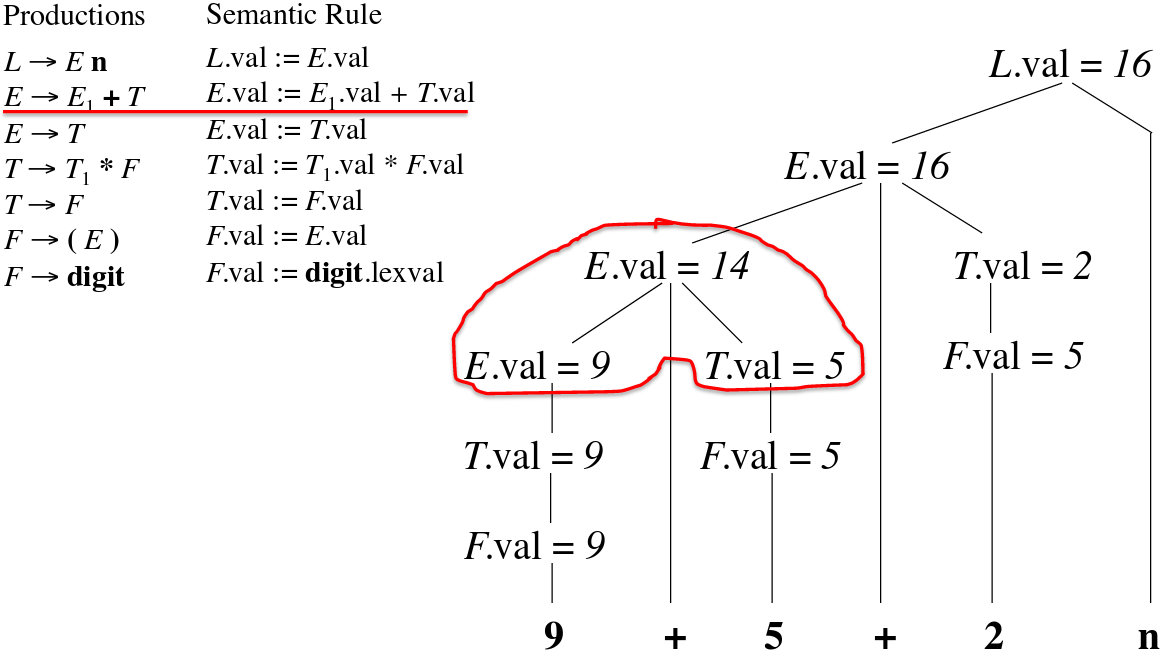
\includegraphics[scale=0.4]{res/image/sdd_example}
  \caption{SDD grammar e albero di parsing annotato}
  \label{img:sdd_example}
\end{figure}

L'attraversamento per la valutazione degli attributi avviene con l'algoritmo di
attraversamento \textit{Depth-First Post-Order} di
fig.\ref{img:traversal_algorithm}.
\begin{figure}[H]
  \centering
  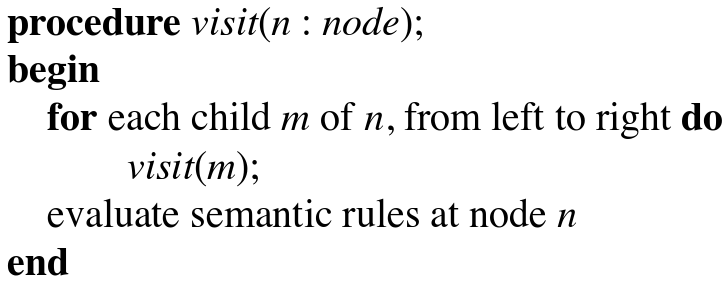
\includegraphics[scale=0.4]{res/image/traversal_algorithm}
  \caption{Algoritmo d'attraversamento Depth-First Post-Order}
  \label{img:traversal_algorithm}
\end{figure}

L'algoritmo va prima a valutare gli attributi figli dei nodi da sinistra verso
destra andando prima sulle foglie, come illustrato in figura

\begin{figure}[H]
  \centering
  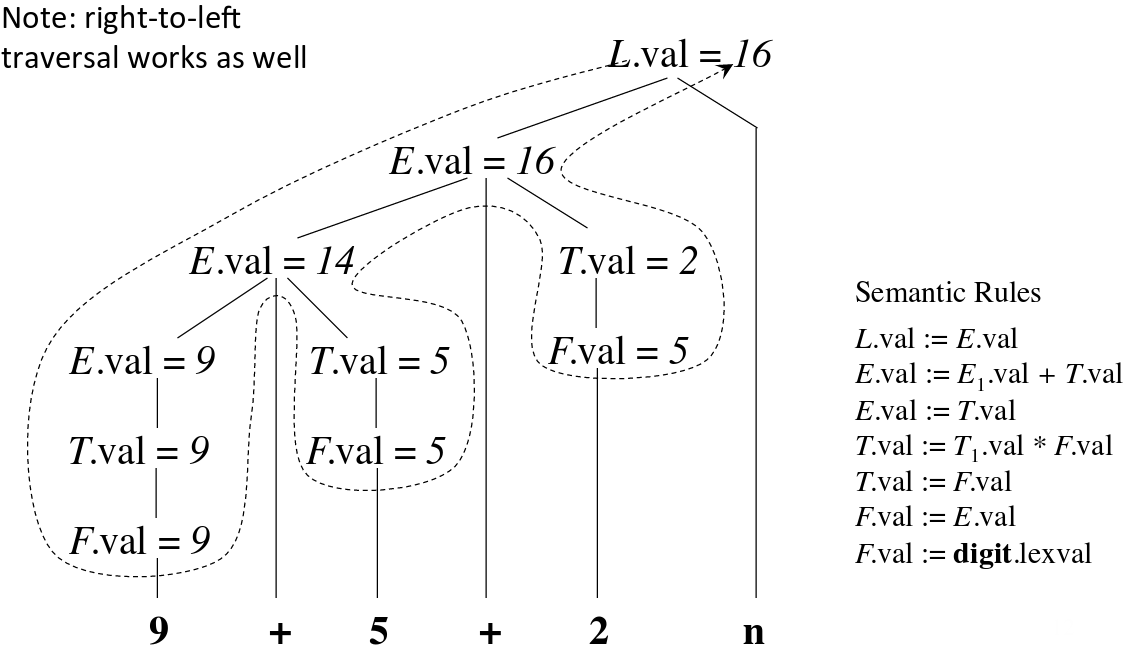
\includegraphics[scale=0.35]{res/image/traversal_tree}
  \caption{Sequenza d'attraversamento dell'albero}
  \label{img:traversal_tree}
\end{figure}

\subsubsection{Generazione di un Abstract Syntax Tree}
Un albero di parsing viene anche chiamato \textit{concrete syntex tree}. L
\textit{abstract syntax tree} \`e scritto dal compilatore per avere una forma
pi\`u di rappresentazione.

Attraverso un \textit{S-attribute definition}, pi\`u precisamente nelle regole
semantiche (fig.\ref{img:semantic_rules}), si va a definire i passi per la
costruzione dell'\textit{abstract syntax tree} a partire dall'albero di parsing
dell'input (fig.\ref{img:build_AST}).

\begin{figure}[H]
  \centering
  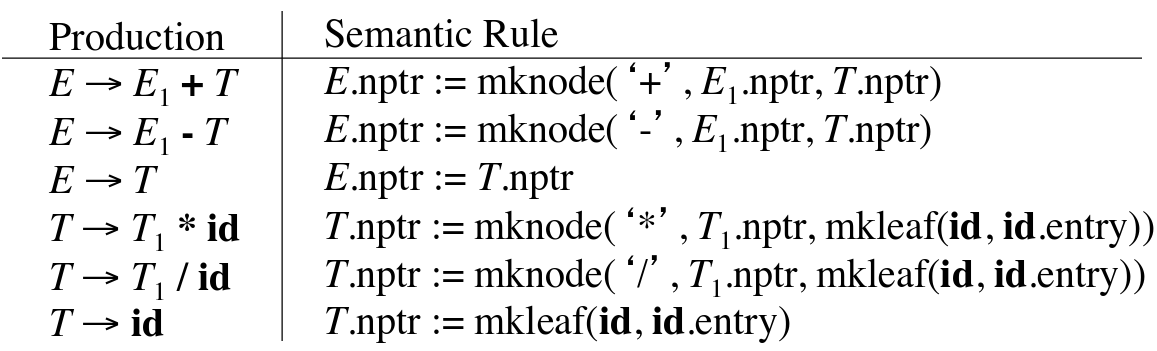
\includegraphics[scale=0.4]{res/image/semantic_rules}
  \caption{Regole semantiche per costruire l'AST}
  \label{img:semantic_rules}
\end{figure}

\begin{figure}[H]
  \centering
  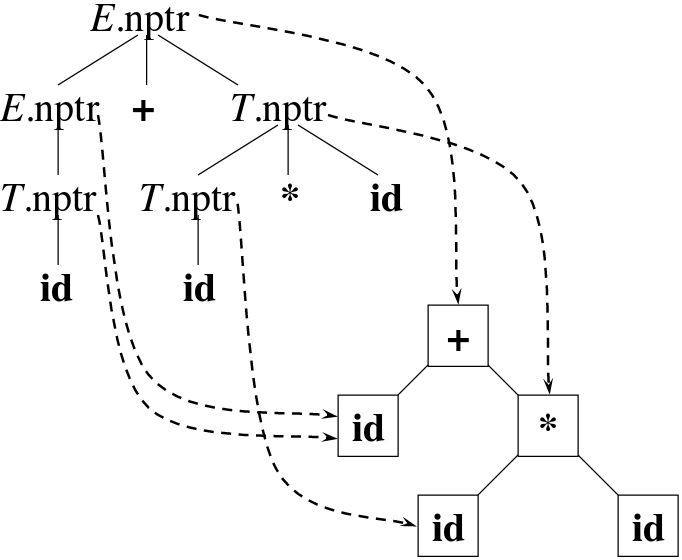
\includegraphics[scale=0.4]{res/image/build_AST}
  \caption{Dal \textit{parse tree} all'AST}
  \label{img:build_AST}
\end{figure}

\subsubsection{Valutazione dell'ordine degli attributi}
In presenza di attributi \textit{inherited} non \`e ovvio in quale ordine gli
attributi dovrebbero essere valutati. Esempio, gli attributi dei non-terminali
in una produzione potrebbero dipendere in modo arbitrario su attributi di altri
simboli (\textbf{non rispettavano} la struttura ad albero).

L'ordina di valutazione deve rispettare alcune dipendenze. Il problema \`e se si
formano dipendenze circolari non c\`e modo di valutare gli attributi.

\subsubsection{Grafico dipendenza per gli attributi}
Dato un albero di sintassi, considerare come nodo tutti i suoi attributi e
rappresentare mediante un grafico tutte le dipendenze \textbf{indotte} dalle
regole semantiche.

\begin{figure}[H]
  \centering
  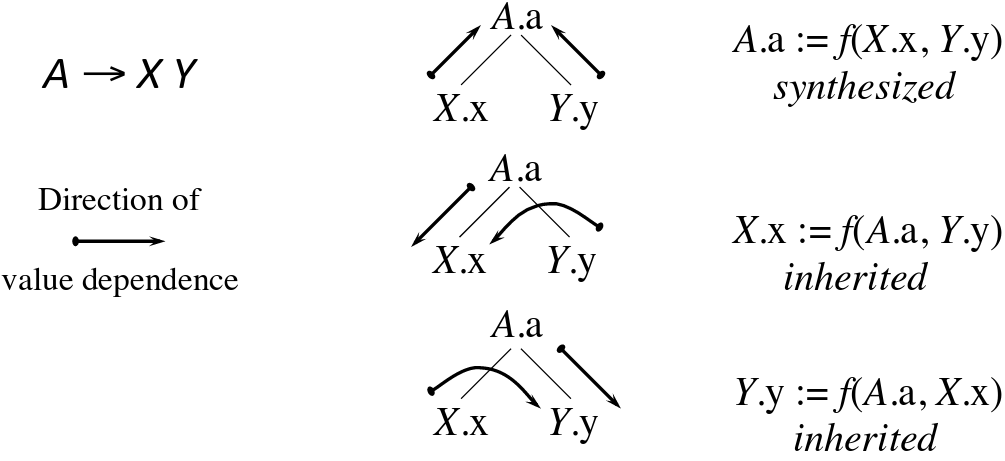
\includegraphics[scale=0.4]{res/image/dependencies_graph}
  \caption{Grafico dipendenze degli attributi}
  \label{img:dependencies_graph}
\end{figure}

Gli spigoli del grafo delle dipendenze \textbf{determinano} l'ordine di
valutazione dei valori degli attributi.

I grafi delle dipendenze \textbf{non possono} essere circolari: impossibile
effettuare la valutazione.
\begin{figure}[H]
  \centering
  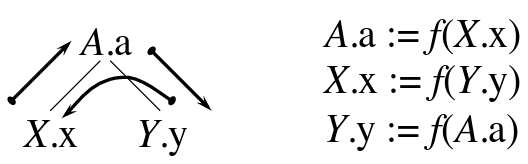
\includegraphics[scale=0.4]{res/image/circular_dependencies}
  \caption{Errore: dipendenze circolari}
  \label{img:circular_dependencies}
\end{figure}

\subsubsection{Topologically Sorted Actions}
\label{sec:evaluation_order}
Dato il grafo delle dipendenze risulta necessario ordinarle in modo da valutare
gli attributi una volta soddisfatte tutte le dipendenze.

\begin{figure}[H]
  \centering
  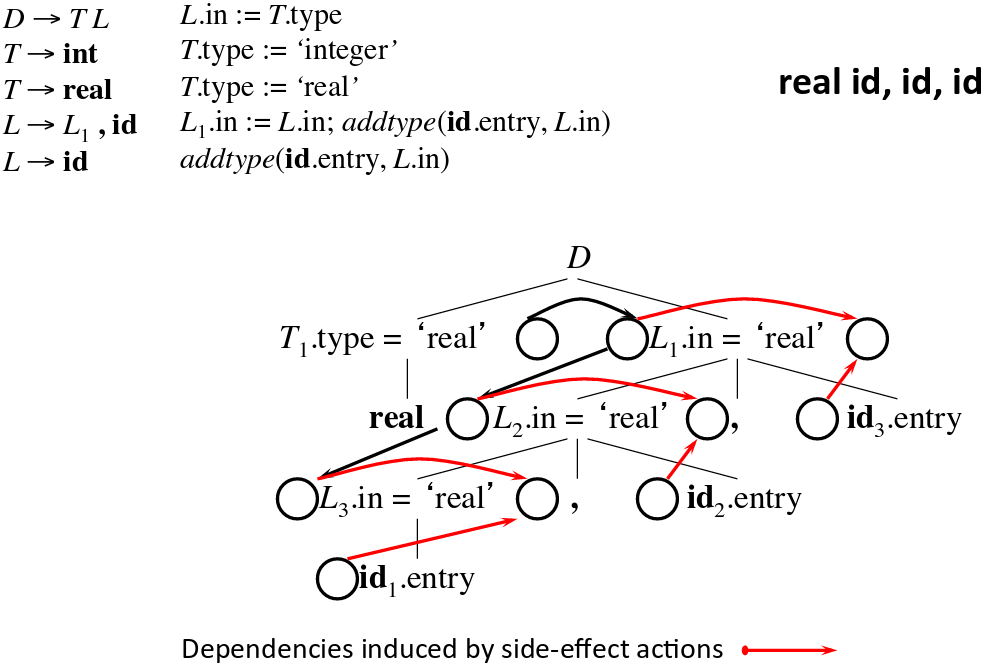
\includegraphics[scale=0.45]{res/image/ex_dependencies}
  \caption{SSD con grafo delle dipendenze}
  \label{img:ex_dependencies}
\end{figure}

\begin{definition}[Topological Sort]
Un topological sort di un grafico direzionato aciclico (DAG) \`e un qualsiasi
ordine $m_1,m_2,...,m_n$ dei nodi del grafo, tale che se $m_i \to m_j$ \`e un
vertice, allora $m_i$ appare prima di $m_j$.
\end{definition}

Ogni topological sort di un grafo delle dipendenze da una valida valutazione
dell'ordine delle regole semantiche.

\begin{figure}[H]
  \centering
  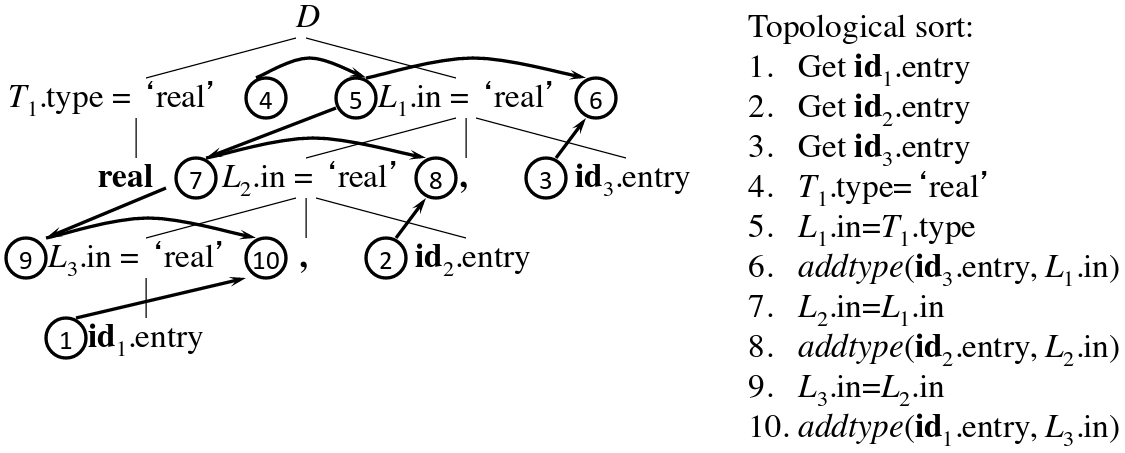
\includegraphics[scale=0.45]{res/image/topological_sort}
  \caption{Valutazione ordine delle dipendenze con il \textit{topological sort}}
  \label{img:topological_sort}
\end{figure}

\subsubsection{Metodo di valutazione}
\paragraph{Parse-tree methods}
Per ogni input, costruire l'albero di parsing ed il grafo delle dipendenze, e
determinare un ordine di valutazione da un \textit{topological sort}.
\paragraph{Rule-base methods}
L'ordine di valutazione \`e determinato dalle regole semantiche.
\paragraph{Oblivious methods}
L'ordine di valutazione \`e fisso e le regole semantiche devono essere
(ri)scritte per supportare l'ordine di valutazione (per esempio S-attributed
definition)

\subsubsection{L-attributed definition}
\begin{definition}[L-attribute definition]
Una syntax-directed definition \`e L-attributed se per ogni attributo
\textbf{inherited} di $X_j$ sul lato destro di $A \to X_1X_2,...,X_n$ dipende
solo da:
\begin{enumerate}
\item gli attributi dei simboli $X_1,X_2,...,X_{j-1}$
\item gli attributi inherited di $A$
\item gli attributi di $X_j$, senza formare dipendenze circolari
\end{enumerate}
\end{definition}

\begin{figure}[H]
  \centering
  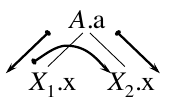
\includegraphics[scale=0.6]{res/image/possible_dependencies}
  \caption{Dipendenze ammesse di attributi \textit{inherited}}
  \label{img:possible_dependencies}
\end{figure}

L-attributed definition permettono, per un ordine naturale, di valutare gli
attributi: \textit{depth-first} e da sinistra a destra.

\begin{figure}[H]
  \centering
  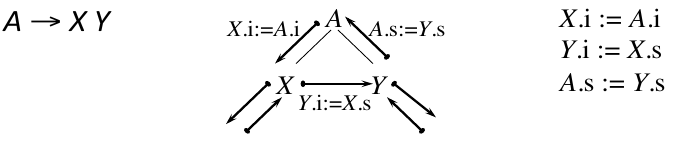
\includegraphics[scale=0.6]{res/image/order_in_Lattributed}
  \caption{Ordine valutazione degli attributi in L-attributed}
  \label{img:order_in_Lattributed}
\end{figure}

\textbf{Ogni S-attributed} \textit{syntex-directed definition} \`e anche
L-attributed, dal momento che non hanno attributi \textit{inherited}.

\subsection{Syntax-Directed Translation Schemes}
Lo schema di transizione provvede una \textbf{notazione alternativa} per le
\textit{Syntex-Directed Definition} e sono molto pi\`u espressive in generale.

Le regole semantiche includo arbitrati \textit{side-effect} e possono
tranquillamente inseriti dentro produzioni.

Le SDD possono essere valutate in \textbf{qualsisasi ordine} compatibile con le
dipendenze; mentre le SDT dovrebbero essere valute da sinistra a destra.

Le SDT possono essere sempre implementate dalla costruzione dell'albero di
derivazione, ed eseguire le azioni ordine \textit{depth-first} da sinistra a
destra.

In alcuni casi l'SDT pu\`o essere implementato durante il parsing, senza
costruire l'interno albero di derivazione prima.

Una produzione di uno \textit{translation scheme} ed il corrispondente nodo in
un albero di derivazione:
\begin{figure}[H]
  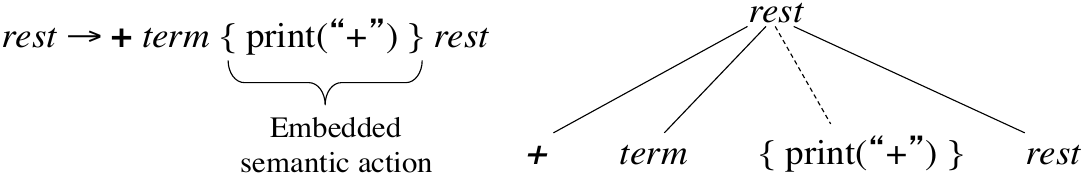
\includegraphics[scale=0.45]{res/image/production_node}
  \caption{Produzione di un SDT ed un nodo di un \textit{parse tree}}
  \label{img:production_node}
\end{figure}

Possibili implementazioni:
\begin{itemize}
\item Costruire l'albero di parsing ignorando le azioni semantiche
\item Aggiungere azioni semantiche nel posto giusto sotto non-terminali
\item Visitare l'albero in \textbf{depth-first, pre-order left-to-right}
eseguendo tutte le azioni
\end{itemize}

\subsubsection{Postfix Translation Schemes}
Se la grammatica \`e LR (perci\`o pu\`o esserle eseguito il parsing
\textit{bottom-up}) e l'SDD \`e S-attributed (attributi solo
\textit{synthesized}), le azioni semantiche possono essere posizionate
\textbf{alla fine della produzione} ed eseguite quando il corpo \`e ridotto alla
testa.

\begin{definition}[Postfix Syntax-Directed Translation]
Syntex-Directed Translation dove tutte le azioni sono alla fine delle produzioni
sono chiamate postfix SDT.
\end{definition}

Un esempio di schema di transizione per notazione postfissa:
\begin{align*}
expr &\to expr + term  & \{print("+")\} \\
expr &\to expr - term  & \{print("-")\} \\
expr &\to term                          \\
term &\to \mathbf{0}   & \{print("0")\} \\
term &\to \mathbf{1}   & \{print("1")\} \\
...  &                 & ...            \\
term &\to \mathbf{9}   & \{print("9")\}
\end{align*}

Se viene dato in input la sequenza \textbf{9-5+2} viene generata la sequenza
\textbf{95-2+} per via dell'attraversamento della fig.\ref{img:postfix_tree}.

\begin{figure}[H]
  \centering
  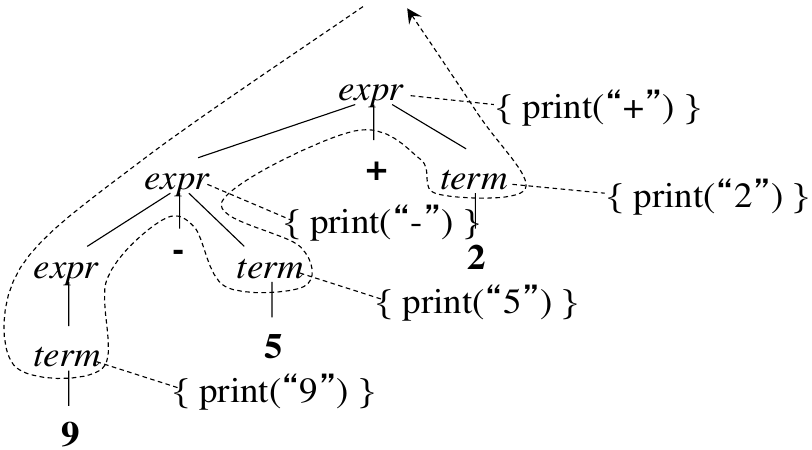
\includegraphics[scale=0.5]{res/image/postfix_tree}
  \caption{Attraversamento dell'albero per notazione postfissa}
  \label{img:postfix_tree}
\end{figure}

\subsubsection{Implementazione di un SDT postfisso}
Le forme postfisse di SDT possono essere implementate durante LR parsing. Le
azioni sono eseguite quando avviene la riduzione, gli attributi possono essere
inseriti nello stack insieme al suo corrispettivo simbolo o stato.

Quando tutti gli attributi sono \textit{synthesized}, l'attributo per la testa
pu\`o essere calcolato al momento della riduzione, essendo che tutti gli
attributi dei simboli del corpo sono gi\`a stati calcolati (per via della
navigazione \textit{depth-first} dell'albero).

\subsubsection{Uso del Translation Schemes per L-Attributed Definitions}
Un \textit{L-attributed} SDD per una grammatica che pu\`o essere analizzata
\textit{top-down} (LL) pu\`o essere implementata usando \textit{Translation
Schemes}:
\begin{enumerate}
\item Inserire le azioni che computano attributi \textbf{inherited} per
non-terminale $A$ prima di $A$
\item Posizionare azioni che computano attributi \textbf{synthesized} per la
testa di una produzione alla fine del corpo di quella produzione
\end{enumerate}

Nota del punto 1: nel \textit{left-to-right parsing}, tutti gli attributi nel
quale l'attributo \textit{inherited} potrebbe dipendere sono gi\`a stati
valutati.

\begin{figure}[H]
  \centering
  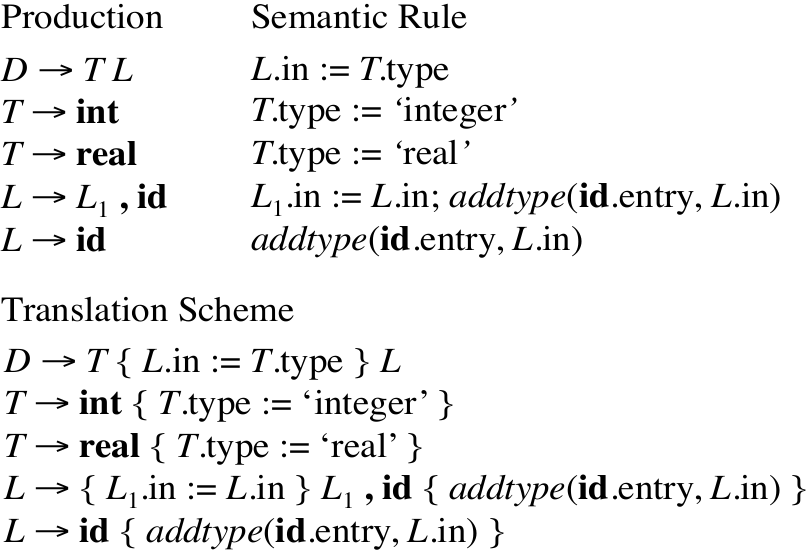
\includegraphics[scale=0.45]{res/image/translation_Lattribute}
  \caption{Definizione del \textit{Translation Scheme}}
  \label{img:translation_Lattribute}
\end{figure}

\subsubsection{Implementare L-attributed Definition}
\paragraph{Parser \textit{Recursive-Descent}}
Nella forma base del parser ogni procedura (associata al simbolo non-terminale)
non aveva ne parametri ne valori di ritorno. Ora per introdurre gli attributi
\textit{synthesized} e \textit{inherited} si fa uso d'entrambi, nello specifico:
\begin{itemize}
\item \textbf{inherited} - attributi \textbf{passati} come argomento
\item \textbf{synthesized} - attributi \textbf{ritornati} come risultato
\end{itemize}

Le procedure immagazzinano gli attributi computati in variabili locali. Per
esempio: date le produzioni
\begin{align*}
D &\to T \ \{L.in:=T.type\} \ L             \\
T &\to \mathbf{int} \ \{T.type:="integer"\} \\
T &\to \mathbf{real} \ \{T.type:="real"\}
\end{align*}
viene eseguito il parser di fig.\ref{img:parser_Lattribute}.

\begin{figure}[H]
  \centering
  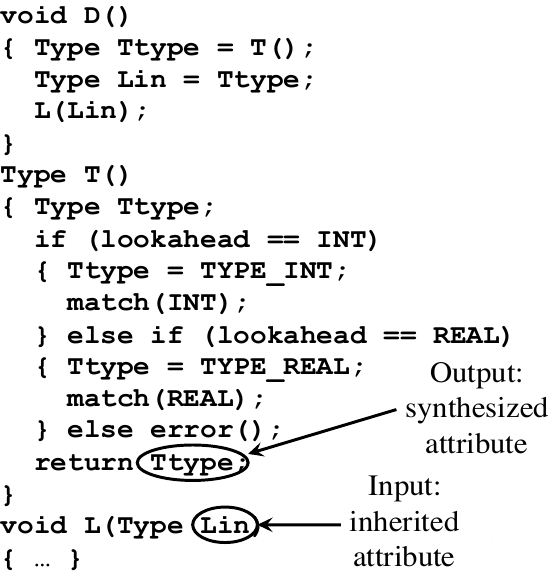
\includegraphics[scale=0.4]{res/image/parser_Lattributed}
  \caption{Parser parziale di un \textit{L-attribute Definition}}
  \label{img:parser_Lattribute}
\end{figure}

\paragraph{Parser \textit{Top-Down Table-Driver}}
Lo stack conterr\`a, a fianco dei simboli della grammatica,
\textit{action-records} e \textit{synthesized-records}.

Gli attributi \textit{inherited} di $A$ sono posizionati nei \textbf{record
di} $A$.

Gli attributi \textit{synthesized} di $A$ sono posizionati nei \textbf{record
appena sotto} $A$.

Sar\`a necessario fare delle copie degli attributi per evitare che siano buttati
fuori dallo stack quando ancora sono necessari.

\paragraph{Parser \textit{Bottom-Up} per grammatiche LL}
Rimuove ogni azione interna con non-terminali marcati:
$A \to \alpha \ \{act\} \ \vartheta \implies$
\begin{align*}
& A \to \alpha N\vartheta \\
& N \to \epsilon \ \{act'\}
\end{align*}
dove $act'$:
\begin{itemize}
\item copia come attributi \textit{inherited} di $N$ ogni attributo di $A$,
$\alpha$ richiesti da $act$
\item calcola attributi come $act$, rendendoli \textit{synthesized} per $N$
\end{itemize}

$act'$ accede ad attributi \textbf{fuori dalla sua produzione}. Questo funziona,
come loro sono (profondamento) nello $LR$ stack.
